\documentclass[10pt]{article}
\usepackage[margin=0.7in]{geometry}
\usepackage{graphicx,booktabs,amsmath,hyperref,mathptmx}
\hypersetup{colorlinks=true,urlcolor=blue}
\title{Setup-charged signed points for actual S3 lifting}
\author{Quadratic-twist study, PR2381}
\date{25 October 2026; signed-cache-20261025}
\begin{document}\sloppy\maketitle
\noindent\textbf{Executed comparison.} C++ and independent Rust execute
80 paired setups and 800 separate nonidentity source recoveries, 40/400 per arm:
ten frozen F43 size-two policies, four direct/transported roles and ten targets.
All 800 scalars verify. Roots, ordered sign lifts, rows/ranks, full solver
certificates, promotions, operational/expanded degrees, failed shifts, base logs
and source answers stay equal. An additional batch-RREF/witness audit checks
all 100 distinct solver certificates. Reference records match the frozen
checked-root route exactly after dropping the new zero counters.

\section*{Cached signs, with setup included}
The cache builds four signed base points, charges two negations, four stored
entries, four canonical/curve checks, four bindings and two inverse-validation
additions once per setup. Every tested lift reads two points and computes its
actual sum. All signs are still tested, even after a successful lift in a query.

\begin{center}\begin{tabular}{lrrrr}\toprule
Prefix policy, separate $Q=P$ & Binary main & Cached main & Binary twist & Cached twist\\\midrule
Setup point-add requests &79&33&73&27\\
Online point-add requests &44&12&61&13\\
Cold point-add requests &125&47&136&42\\
Cold negation requests &20&2&24&2\\
Cold scalar-loop iterations &54&14&56&8\\
Cold cache reads &0&40&0&48\\
Tested signed lifts &20&20&24&24\\
Represented matrix slots &540&540&36&36\\\bottomrule
\end{tabular}\end{center}
All 400 candidate cold records have fewer point-add requests than their own
reference, including cache validation. With $L$ tested lifts, the exact delta
is $-4L+2$ in setup/cold and $-4L$ online. Negations change by $-L+2$
(setup/cold), scalar iterations by $-2L$, and cache reads by $+2L$.
Other old components are unchanged. Ratios $125/47$ and $136/42$ describe
point-add requests, \emph{not speedups}.

\noindent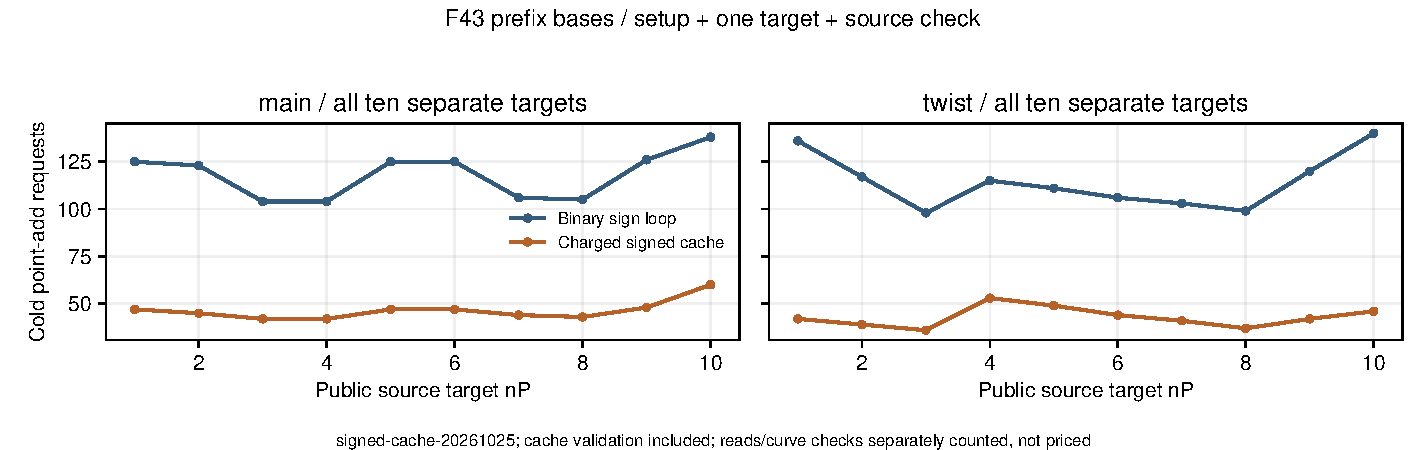
\includegraphics[width=\linewidth]{lifting.pdf}

\noindent\textbf{Reference quality matters.} The old binary sign loop includes
unused final doublings and identity additions. Compilers may optimize unused
arithmetic. These36 unpriced components are algorithm requests, not retired
instructions or runtime. Cache storage/reads, curve-check coordinate work,
field tables, allocation, sorting/traversal, hashing and audit remain unpriced.
Direct uncached signs are the next stronger reference. No calibrated total,
GAE, $S$, rho, intrinsic regularity or fastest-external claim is admitted.

\newpage
\section*{Validation implies exactly the old lifting rule}
In an additive commutative group, validation requires
\[
 C_i(+) = B_i,\qquad C_i(-)+B_i=O.
\]
Lean derives $C_i(-)=-B_i$, then proves equality of cached and scalar signed
sums and of \emph{ordered filtered candidate lists}, preserving order and
duplicates. Arbitrary indices may repeat. A cached relation to the shifted
target yields source recovery through an injective additive map; reduction
modulo$r$ explicitly uses the source annihilator $rP=O$.

The actual F43 twist cache is $(15,9),(17,6)$ and negatives $(15,34),(17,37)$.
Mathlib nonsingular points, inverse checks and base logs $B_0=5U,B_1=7U$ are
kernel checked. The concrete recovery theorem requires the actual target
relation, but assumes neither cache correctness nor the base logs.

\begin{center}\begin{tabular}{lp{0.60\linewidth}}\toprule
Claim & Declaration in \texttt{SignedCache}\\\midrule
Sign and validated cache & \texttt{signed\_eq\_zsmul}, \texttt{validated\_cache\_value}\\
Pair sums and ordered lifts & \texttt{cached\_sum\_eq}, \texttt{ordered\_lifts\_eq}\\
Shifted source recovery & \texttt{cached\_relation\_recovers\_mod}\\
Actual F43 checks & \texttt{F43.actual\_cache\_valid}, \texttt{actual\_base\_logs}, \texttt{actual\_cached\_recovery}\\
Coordinate inverse & \texttt{coordinate\_inverse}\\\bottomrule
\end{tabular}\end{center}
Nine new public theorems; unmodified scoped gate 191 public /249 audited,
zero failing/extra trusted axioms. Only propext, Classical.choice and Quot.sound.
Certificate \texttt{IDC1h202bb532af10c977} checks only $y+(-y)=0$ at 32+16 points,
with false identity/source rejection. Group/list/recovery claims rest on Lean,
while native execution and request vectors are independently replayed.

\noindent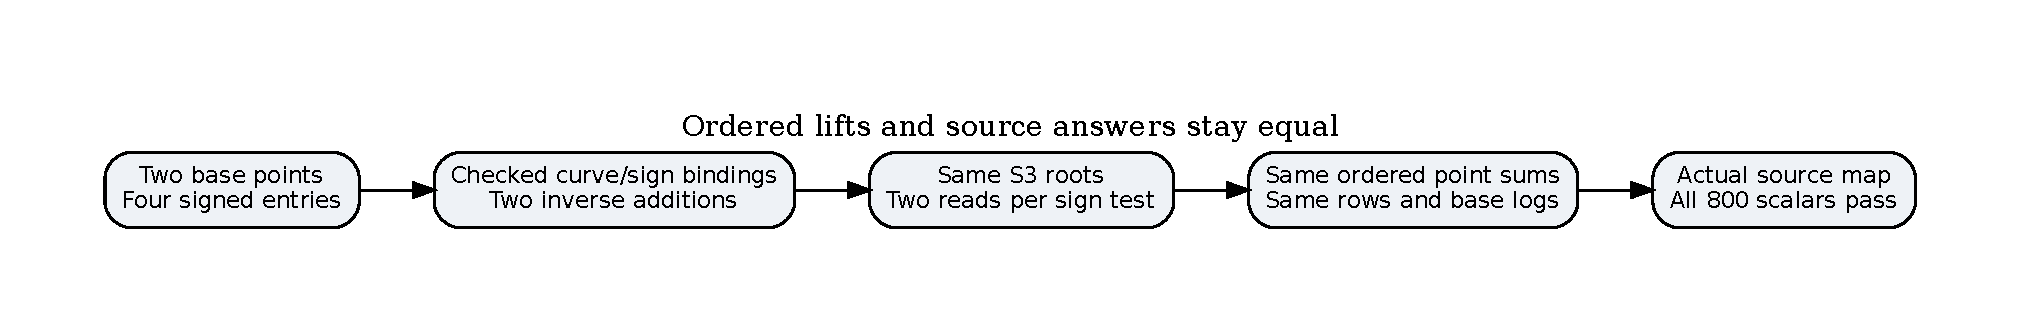
\includegraphics[width=\linewidth]{bridge.pdf}

\section*{All policies, actual map and limitations}
Across 100 unmatched cached main/twist records, twist point-add requests are
lower/equal/higher in 43/1/56, matrix slots 44/15/41, scalar iterations 33/10/57.
Summed hypothetical cold additions are 4398/4638, versus 11750/11990 before;
these sum separate one-target records, not batch throughput. Transported bases
match every component except explicit coordinate maps. Later losses remain.

Models \texttt{icv1-fp6-t0-74779950} and \texttt{icv1-fp6-t0-c6a8a47c} are
$E:y^2=x^3+x$ and $T:Y^2=X^3+4X$ over F43, order-11 generators$(31,18)$
and$(24,26)$. The actual map$(x,y)\mapsto(41x,11y)$ binds the source DLP.
This is an exceptional base-field-isomorphic fixture; the new generator has
no EC1 registration. Recovery receives only the source point. Earlier first
query rank0/2 and operational degree3/2 remain, with equal homogeneous cutoff2.

Seven rehashed controls reject without receipt, including an on-curve point
in the wrong sign slot. The exact fresh replay and 22 backend tests pass.
Both proof drafts/logs remain; final proofs generalize the first compiled
fixed-column draft before native execution. Profile probe lacks gawk, Conductor
exits127, and no upload or paid resource occurred. Next compare direct uncached
signs on the same targets. Calibration, general geometry, stationary useful
yield, review, exact-head CI access and integration remain open.
Full sources, proof map, commands and validation are linked in the README.
\end{document}
